\documentclass[a4paper,11pt]{article}
\usepackage[utf8]{inputenc}
\usepackage[spanish]{babel}
\usepackage[affil-it]{authblk}
\usepackage{enumerate}
\usepackage{graphicx}
\usepackage{hyperref}
\usepackage{amsmath}
\usepackage{amssymb}
\usepackage{cancel}
\usepackage[usenames, dvipsnames]{color}
\usepackage{tikz}
\usepackage[labelfont=bf]{caption}
\usepackage{subcaption} %Multiple images
\usepackage{multicol} % Multiple columns
\usepackage{float}
\usepackage{cleveref}
\usepackage{relsize} % bigger math symbols
\usepackage[margin=1.1in]{geometry}
\usepackage[titletoc,toc,title]{appendix}
\usepackage{enumitem}
\usepackage{etoolbox}
\usepackage{mdframed} %frame theorems
\usetikzlibrary{calc}
\numberwithin{equation}{section}

% Footnotes with symbols

\makeatletter
\def\@fnsymbol#1{\ensuremath{\ifcase#1\or \dagger\or \ddagger\or
   \mathsection\or \mathparagraph\or \|\or **\or \dagger\dagger
   \or \ddagger\ddagger \else\@ctrerr\fi}}
\makeatother

\renewcommand{\thefootnote}{\fnsymbol{footnote}}

% Cool letters 
%Filename:      Typocaps.fd
%Created by:    MLO
%Creation date: 2003/04/02

% This file should be put in a TeX input directory

\ProvidesFile{Typocaps.fd}
   [2003/04/02 Font definition file for U/Typocaps]

\DeclareFontFamily{U}{Typocaps}{}

\DeclareFontShape{U}{Typocaps}{xl}{n}{
   <-> Typocaps
}{}

\endinput


% Footer
\usepackage{fancyhdr}
\pagestyle{fancy}
\fancyhf{}
\cfoot{\fontsize{15pt}{15pt}\usefont{U}{Typocaps}{xl}{n} 
gigantium humeris insidentes}

% Big Pictures
\usepackage[export]{adjustbox}

% Enviroment for theorems
\newmdtheoremenv[frametitle=Teorema]{theo}{Theorem}

% Circled words
\newcommand{\circled}[2][]{%
  \tikz[baseline=(char.base)]{%
    \node[shape = circle, draw, inner sep = 1pt]
    (char) {\phantom{\ifblank{#1}{#2}{#1}}};%
    \node at (char.center) {\makebox[0pt][c]{#2}};}}
\robustify{\circled}

%Appendices in spanish
\renewcommand{\appendixname}{Ap\'endices}
\renewcommand{\appendixtocname}{Ap\'endices}
\renewcommand{\appendixpagename}{Ap\'endices}

%Zero delimiter
\newcommand{\zerodel}{.\kern-\nulldelimiterspace}

%Columns separation
\setlength{\columnsep}{1cm}

%Indentation
\setlength{\parindent}{0ex}

%Multiple References

\crefrangelabelformat{equation}{(#3#1#4--#5\crefstripprefix{#1}{#2}#6)}

\usepackage{xparse}

%Boxes

\newcommand*{\boxcolor}{blue}
\makeatletter
\renewcommand{\boxed}[1]{\textcolor{\boxcolor}{%
\tikz[baseline={([yshift=-1ex]current bounding box.center)}] \node [rectangle, minimum width=1ex,rounded corners,draw] {\normalcolor\m@th$\displaystyle#1$};}}
 \makeatother

%Constantes
\newcommand{\euler}{\mathrm{e}}
\newcommand{\im}{i}

%Lemas, teoremas, definiciones y pruebas
\newcommand{\definicion}{\textbf{Definición: }}
\newcommand{\lema}{\textbf{Lema: }}
\newcommand{\teorema}{\textbf{Teorema: }}
\newcommand{\prueba}{\textbf{Prueba: }}
\newcommand{\proposicion}{\textbf{Proposición: }}
\newcommand{\corolario}{\textbf{Corolario: }}

% Definición de las secciones y su numeración

\makeatletter
\def\@seccntformat#1{%
  \expandafter\ifx\csname c@#1\endcsname\c@section\else
  \csname the#1\endcsname\quad
  \fi}
\makeatother

\begin{document}

\begin{titlepage}
\thispagestyle{fancy}

\newcommand{\HRule}{\rule{\linewidth}{0.5mm}} % Defines a new command for the horizontal lines, change thickness here

\center % Center everything on the page
 
%----------------------------------------------------------------------------------------
%	HEADING SECTIONS
%----------------------------------------------------------------------------------------

\textsc{\LARGE Universidad Nacional Autónoma de México}\\[0.3cm] % Name of your university/college

%----------------------------------------------------------------------------------------
%	LOGO SECTION
%----------------------------------------------------------------------------------------

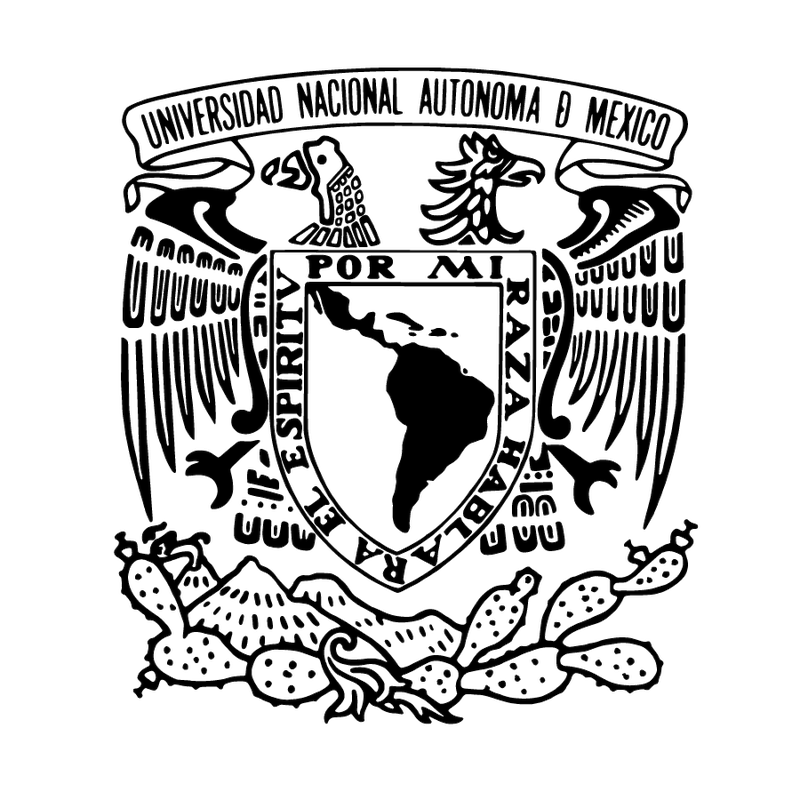
\includegraphics[scale=0.17]{unam}

%----------------------------------------------------------------------------------------
%	SUBHEADING SECTIONS
%----------------------------------------------------------------------------------------

\textsc{\Large Electrodinámica Clásica}\\[0.5cm] % Major heading such as course name
\textsc{\large Semestre 2016-II}\\[0.5cm] % Minor heading such as course title

%----------------------------------------------------------------------------------------
%	TITLE SECTION
%----------------------------------------------------------------------------------------

\HRule \\[0.4cm]
{ \huge \bfseries Tarea \# 1. \\ Introducción a al 
Electrostática.}\\[0.2cm] % Title of your document
\HRule \\[0.2cm]
 
%----------------------------------------------------------------------------------------
%	AUTHOR SECTION
%----------------------------------------------------------------------------------------
\setcounter{footnote}{0}
\center
\large
\emph{Autor:} \\ % Your name
\Large Favio \textsc{Vázquez}\footnote[1]{\href{mailto:favio.vazquez@correo.nucleares.unam.mx}{favio.vazquez@correo.nucleares.unam.mx}}

%----------------------------------------------------------------------------------------
%	COOL IMAGE SECTION
%----------------------------------------------------------------------------------------

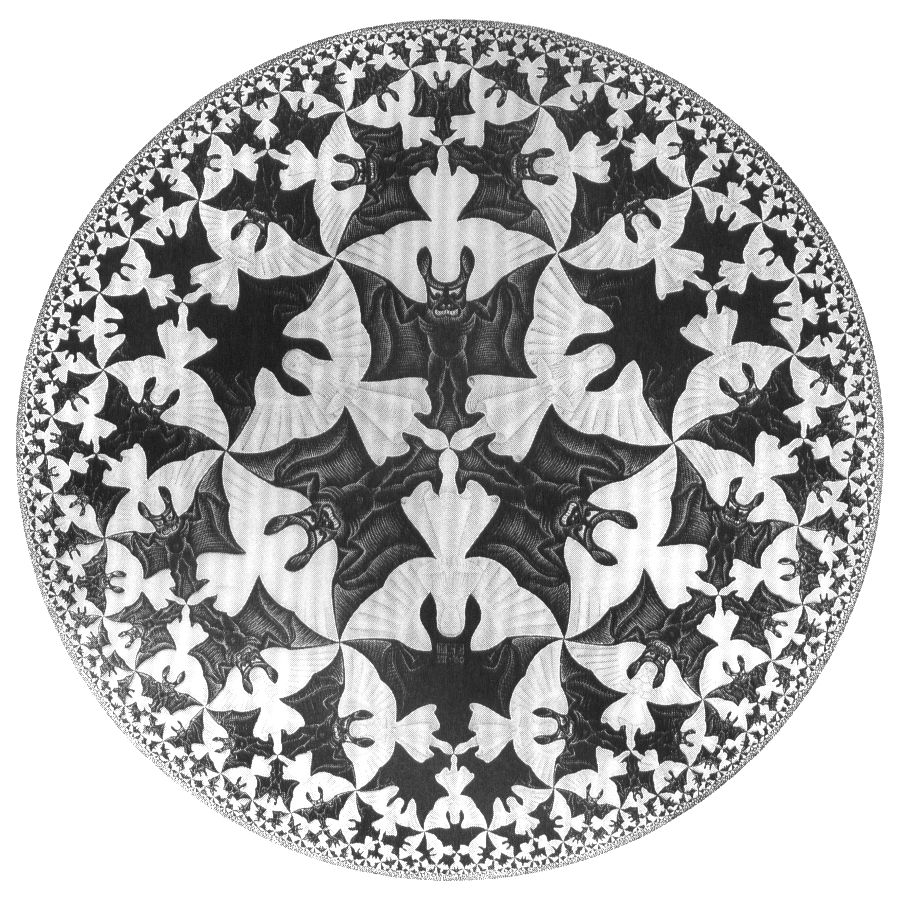
\includegraphics[scale=0.35]{angelsDemonsEscher}

%----------------------------------------------------------------------------------------

\vfill % Fill the rest of the page with whitespace

\end{titlepage}

% ---------------------------------------------------------------------------------------
%         HEADER
%----------------------------------------------------------------------------------------

\fancyhead[L]{Favio Vázquez}
\fancyhead[R]{\thepage}

%----------------------------------------------------------------------------------------
\setcounter{footnote}{0}
\renewcommand*{\thefootnote}{\arabic{footnote}}

\section{Problema 1. Problema 1.2 de Classical Electrodynamics (3ra ed) de 
Jackson \cite{jackson}.}

La función delta de Dirac en tres dimensiones puede tomarse como el límite impropio 
mientras $\alpha \rightarrow 0$ de la función gaussiana 

$$
D(\alpha;x,y,z) = (2\pi)^{-3/2}\alpha^{-3}\exp\left[-\frac{1}{2a}(x^2 + y^2 + z^2) \right].
$$

Considere un sistema de coordenadas ortogonal general especificado por las superficies 
$u = \text{constante}$, $v = \text{constante}$, $w = \text{constante}$, con elementos 
de longitud $du/U$, $dv/V$, $dw/W$ en las tres direcciones perpendiculares. Mostrar 
que

$$
\delta(\mathbf{x} - \mathbf{x}') = \delta(u - u')\delta(v - v')\delta(w - w')\cdot UVW
$$

considerando el límite de la gaussiana de arriba. Note que mientras $\alpha \rightarrow 
0$, sólo el elemento de longitud infinitesimal necesita ser usado para la distancia
entre los puntos en la exponencial.

\vspace{.3cm}

\underline{Solución:} \vspace{.3cm}

Partiendo de la ecuación 

\begin{equation}
 D(\alpha;x,y,z) = (2\pi)^{-3/2}\alpha^{-3}
 \exp\left[-\frac{1}{2a}(x^2 + y^2 + z^2) \right],
\end{equation}

y haciendo el cambio de variable $x \rightarrow x-x'$, $y \rightarrow y-y'$, 
$z \rightarrow z-z'$ obtenemos 

\begin{equation*}
 D(\alpha;x-x',y-y',z-z') = (2\pi)^{-3/2}\alpha^{-3}
 \exp\left\{-\frac{1}{2a}[(x-x')^2 + (y-y)^2 + (z-z')^2] \right\}.
\end{equation*}

Notamos que mientras $\alpha \rightarrow 0 \Rightarrow D \rightarrow 0$, a 
menos que  $x \rightarrow x-x'$, $y \rightarrow y-y'$, $z \rightarrow z-z' 
\rightarrow 0$ también. Y recordando que $x-x' \rightarrow 0 \Rightarrow dx$, etc., 
tenemos 

\begin{equation}
 D(\alpha;x-x',y-y',z-z') = (2\pi)^{-3/2}\alpha^{-3}
 \exp\left[-\frac{1}{2a}(dx^2 + dy^2 + dz^2) \right].
\end{equation}

Recordamos también que el elemento de longitud se escribe como, 

\begin{equation}
 ds^2 = dx^2 + dy^2 + dz^2,
\end{equation}

entonces 

\begin{equation}
 D(\alpha;x-x',y-y',z-z') = (2\pi)^{-3/2}\alpha^{-3}
 \exp\left[-\frac{1}{2a}(ds^2) \right].
 \label{eq:15}
\end{equation}

Y utilizando el sistema de coordenadas que hay que considerar según el problema, 
podemos reescribir $ds^2$ como 

\begin{equation}
 ds^2 = \left(\frac{du}{U}\right) + \left(\frac{dv}{V}\right) + 
 \left(\frac{dw}{W}\right),
\end{equation}

donde recalcamos que no estamos diciendo que $dx = du/U$, etc., sino que estamos 
usando el hecho de que $ds^2$ es el mismo en todos los sistemas ortogonales, 
por lo tanto podemos reescribir \eqref{eq:15} como 

\begin{equation}
 D(\alpha;u,v,w) = (2\pi)^{-3/2}\alpha^{-3}
 \exp\left[-\frac{1}{2\alpha^2}\left(\frac{du^2}{U^2} + 
 \frac{dv^2}{V^2} + \frac{dw^2}{W^2}\right) \right].
\end{equation}

Ahora expandimos de vuelta los diferenciales en diferencias, 

\begin{equation*}
 D(\alpha;u-u',v-v',w-w') = (2\pi)^{-3/2}\alpha^{-3}
 \exp\left\{-\frac{1}{2\alpha^2}\left[\frac{(u - u')^2}{U^2} + 
 \frac{(v-v')^2}{V^2} + \frac{(w-w')^2}{W^2}\right] \right\},
\end{equation*}

que podemos escribir como (utilizando el hecho que $\exp(a+b) = \exp(a)\exp(b)$),

\begin{equation*}
 D = (2\pi)^{-3/2}\alpha^{-3}
 \exp\left[-\frac{1}{2\alpha^2}\frac{(u - u')^2}{U^2}\right]
 \exp\left[-\frac{1}{2\alpha^2}\frac{(v-v')^2}{V^2}\right]
 \exp\left[-\frac{1}{2\alpha^2}\frac{(w-w')^2}{W^2}\right],
\end{equation*}

y esta ecuación puede expresarse de una forma más conveniente como 

\begin{equation}
 D = \frac{\exp\left[-\frac{1}{2\alpha^2}\frac{(u - u')^2}{U^2}\right]}{\sqrt{2\pi}\alpha}
 \frac{\exp\left[-\frac{1}{2\alpha^2}\frac{(v-v')^2}{V^2}\right]}{\sqrt{2\pi}\alpha}
 \frac{\exp\left[-\frac{1}{2\alpha^2}\frac{(w-w')^2}{W^2}\right]}{\sqrt{2\pi}\alpha}.
\label{eq:110}
\end{equation}

La cual es una ecuación que comienza a parecerse a la definición de la delta. Ahora 
si reemplazamos en cada término del lado derecho de \eqref{eq:110} las $\alpha$'s 
por $\alpha_u/U$, $\alpha_v/V$ y $\alpha_w/W$ respectivamente\footnote{Podemos 
hacer esto si $\alpha_u,\alpha_v,\alpha_w \rightarrow 0$ mientras que 
$\alpha \rightarrow 0$.} y obtenemos 

\begin{equation}
 D(\alpha;u-u',v-v',w-w') = \frac{\exp\left[-\frac{(u - u')^2}{2\alpha_u}\right]}{\sqrt{2\pi}\alpha}
 \frac{\exp\left[\frac{(v-v')^2}{2\alpha_v}\right]}{\sqrt{2\pi}\alpha}
 \frac{\exp\left[\frac{(w-w')^2}{2\alpha_w}\right]}{\sqrt{2\pi}\alpha}\cdot UVW.
 \label{eq:112}
\end{equation}

Ahora tomando el límite mientras $\alpha_u,\alpha_v,\alpha_w \rightarrow 0$, 
vemos que cada término del lado derecho de \eqref{eq:112} se convierte en un 
delta de Dirac unidimensional y el lado izquierdo en la expresión 
general de la delta de Dirac tridimensional, por lo tanto \eqref{eq:112} se 
transforma en 

\begin{equation*}
 \boxed{\underset{\alpha_u,\alpha_v,\alpha_w \rightarrow 0}{\text{lím}} 
 D(\alpha;u-u',v-v',w-w') = \delta(\mathbf{x} - \mathbf{x}') = 
 \delta(u - u')\delta(v - v')\delta(w - w')\cdot UVW.}
\end{equation*}

\newpage

\section{Problema 2. Problema 1.3 de Classical Electrodynamics (3ra ed) de 
Jackson \cite{jackson}.}

Usando las funciones delta de Dirac en las coordenadas apropiadas, exprese las 
siguientes distribuciones de carga como las densidades de carga tridimensionales 
$\rho(\mathbf{x}).$

\begin{enumerate}[label=\textbf{(\alph*)}]
 \item En coordenadas esféricas, una carga $Q$ uniformemente distribuida sobre 
 una concha esférica de radio $R$.
 \item En coordenadas cilíndricas, una carga $\lambda$ por unidad de longitud 
 uniformemente distribuida sobre una superficie cilíndrica de radio $b$.
 \item En coordenadas cilíndricas, una carga Q extendida uniformemente sobre 
 un disco plano de grosor despreciable y radio $R$.
 \item Lo mismo que en la parte \textbf{(c)}, pero usando coordenadas esféricas.
\end{enumerate}

\vspace{.3cm}

\underline{Solución:} \vspace{.3cm}

El método que utilizaremos para solucionar cada caso será usar el hecho de que 
la densidad de carga en cada caso, será proporcional a una delta de Dirac. Luego 
utilizaremos la propiedad de que dos objetos proporcionales se pueden escribir 
como el uno igual al otro multiplicado por un parámetro arbitrario, luego integraremos sobre 
el objeto completo, igualaremos a la carga total y resolveremos para el parámetro 
arbitrario.

\vspace{.3cm}

Recordamos que 

\begin{equation}
 Q = \int \rho(\mathbf{x})d^3x.
\end{equation}

\textbf{(a)} Para una carga $Q$ distribuida uniformemente sobre una concha esférica, 
sabemos que la distribución de carga se puede escribir como 

\begin{equation}
 \rho(\mathbf{x}) = \rho(r,\theta,\phi) \propto \delta(r-R),
\end{equation}

\begin{equation}
 \rho(\mathbf{x}) =  \rho(r,\theta,\phi) = \xi(R)\delta(r-R),
\end{equation}

donde $\xi(R)$ es el parámetro arbitrario a determinar. Entonces, recordando que 
en coordenadas esféricas $d^3x = r^2\sen{\theta}dr d\theta d\phi$, 

\begin{equation*}
 Q = \int_0^{2\pi} \int_0^\pi \int_0^\infty 
  \rho(r,\theta,\phi) r^2\sen{\theta}dr d\theta d\phi = 
  \int_0^{2\pi} \int_0^\pi \int_0^\infty \xi(R)\delta(r-R)
  r^2\sen{\theta}dr d\theta d\phi,
\end{equation*}

\begin{equation}
 Q = 4\pi\xi(R) \int_0^\infty \delta(r-R) r^2dr = 4\pi R^2 \xi(R),
\end{equation}

\begin{equation}
\therefore \xi(R) = \frac{Q}{4\pi R^2}.
\end{equation}

Entonces, 

\begin{equation}
 \boxed{\rho(\mathbf{x}) =  \rho(r,\theta,\phi) = \frac{Q}{4\pi R^2}\delta(r-R)}.
\end{equation}

\vspace{.3cm}

Que era lo esperado, la densidad de carga es la carga total dividida por el área de
la esfera por la delta.

\vspace{.3cm}

\textbf{(b)} Para la superficie cilíndrica, 

\begin{equation}
 \rho(\mathbf{x}) =  \rho(r,\theta,z) \propto \delta(r - b),
\end{equation}

\begin{equation}
 \rho(\mathbf{x}) =  \rho(r,\theta,z) = \xi(b) \delta(r - b),
\end{equation}

donde $\xi(b)$ es el parámetro arbitrario a determinar. Entonces, recordando que 
en coordenadas cilíndricas $d^3x = rdr d\theta$, 

\begin{equation*}
 \lambda = \int_0^{2\pi} \int_0^\infty 
  \rho(r,\theta,\phi) rdr d\theta = 
  \int_0^{2\pi} \int_0^\infty \xi(b)\delta(r-b)
  r drd\theta,
\end{equation*}

\begin{equation}
 \lambda = \xi(b)2\pi \int_0^\infty \delta(r-b)rdr = \xi(b)2\pi,
\end{equation}

\begin{equation}
 \therefore \xi(b) = \frac{\lambda}{2\pi b}.
\end{equation}

Entonces, 

\begin{equation}
 \boxed{\rho(\mathbf{x}) =  \rho(r,\theta,z) = \frac{\lambda}{2\pi b}\delta(r - b)}.
\end{equation}

Que era lo esperado, la densidad de carga es la carga total dividida por la circunferencia 
del cilindro por la delta.

\vspace{.3cm}

\textbf{(c)} Para el disco plano, debemos usar la función de paso $H$ en la dirección 
radial, 

\begin{equation}
 \rho(\mathbf{x}) =  \rho(r,\theta,z) \propto \delta(z)H(R-r),
\end{equation}

\begin{equation}
 \rho(\mathbf{x}) =  \rho(r,\theta,z) = \xi(R) \delta(z)H(R-r),
\end{equation}

donde $\xi(R)$ es el parámetro arbitrario a determinar. Entonces, recordando que 
en coordenadas cilíndricas $d^3x = rdr d\theta$, 

\begin{equation*}
 Q = \int_{-\infty}^{\infty}\int_0^{2\pi} \int_0^\infty 
  \rho(r,\theta,\phi) rdr d\theta dez = 
  \int_{-\infty}^{\infty} \int_0^{2\pi} \int_0^\infty \xi(R) \delta(z)H(R-r)
  r drd\theta dz,
\end{equation*}

\begin{equation}
 Q = \xi(R) \cancelto{1}{\int_{-\infty}^{\infty} \delta(z)dz} 
 \cancelto{2\pi}{\int_0^{2\pi} d\theta}
 \int_0^\infty H(R-r) r dr = \xi(R) 2\pi \int_0^R rdr,
\end{equation}

\begin{equation}
 \therefore \xi(b) = \frac{Q}{\pi R^2}.
\end{equation}

Entonces, 

\begin{equation}
 \boxed{\rho(\mathbf{x}) =  \rho(r,\theta,z) = \frac{Q}{\pi R^2}\delta(z)H(R-r)}.
\end{equation}

Que también era lo esperado, la densidad de carga es la delta por la densidad de 
carga superficial, que en este caso es la carga total dividida por el área del 
disco.

\vspace{.3cm}

\textbf{(c)} Para el disco plano en coordenadas esféricas, es lo mismo que el caso 
anterior, pero en este caso confinado al plano $z$, que es lo mismo que decir que 
$\theta = \pi/2$. Entonces, 

\begin{equation}
 \rho(\mathbf{x}) =  \rho(r,\theta,\phi) \propto 
 \frac{\delta(\theta - \pi/2)}{r}H(R-r),
\end{equation}

\begin{equation}
 \rho(\mathbf{x}) =  \rho(r,\theta,\phi)  = 
 \xi(R)\frac{\delta(\theta - \pi/2)}{r}H(R-r),
\end{equation}

donde $\xi(R)$ es el parámetro arbitrario a determinar. Entonces, recordando que 
en coordenadas esféricas $d^3x = r^2\sen{\theta}dr d\theta d\phi$,

\begin{align*}
 Q &= \int_0^{2\pi} \int_0^\pi \int_0^\infty 
  \rho(r,\theta,\phi) r^2\sen{\theta}dr d\theta d\phi \\
  &=   \xi(R)\int_0^{2\pi}d\phi \int_0^\pi \delta(\theta - \pi/2)\sen{\theta}d\theta 
  \int_0^\infty H(R-r)rdr,
\end{align*}

\begin{equation}
 \therefore \xi(R) = \frac{Q}{\pi R^2}.
\end{equation}

Entonces,

\begin{equation}
 \boxed{\rho(r,\theta,\phi) = \frac{Q}{\pi R}\frac{\delta(\theta - \pi/2)}{r}H(R-r)}.
\end{equation}

\newpage

\section{Problema 3. Problema 1.4 de Classical Electrodynamics (3ra ed) de 
Jackson \cite{jackson}.}

Cada una de las esferas cargadas de radio $a$, una conductora, una con una densidad 
de carga uniforme adentro de su volumen, y una con una densidad de carga esféricamente 
simétrica que varía radialmente como $r^n$ ($n > -3)$, tiene una carga total $Q$. 
Use el teorema de Gauss para obtener los campos eléctricos tanto adentro como afuera 
de la esfera. Esboce el comportamiento de los campos como una función del radio 
para las primeras dos esfera, y para la tercera com $n= -2,+2$. 

\vspace{.3cm}

\underline{Solución:} \vspace{.3cm}

\textbf{(a)} En el primer caso tenemos una esfera conductora. Primero recordamos que 
dentro de la esfera el campo eléctrico es cero. Para obtener el campo eléctrico 
fuera de la esfera, procedemos como siempre a dibujar una esfera concéntrica de 
integración con un radio $r$, como es muy simple el problema solo nos planteamos 
el procedimiento mentalmente. Recordando la forma integral de la ley de Gauss,

\begin{equation}
 \oint_S \mathbf{E} \cdot d\mathbf{A} = \frac{Q}{\epsilon_0},
\end{equation}

y debido a la simetría entre la esfera conductora y la esfera, el campo eléctrico es 
constante sobre la superficie de integración y entonces podemos escribir:

\begin{equation}
  E \oint_S  d\mathbf{A} = \frac{Q}{\epsilon_0}.
\end{equation}

Debemos evaluar la integral de superficie sobre el área total de integración 
de la esfera de radio $r$, por lo tanto 

\begin{equation}
 E4\pi r^2 = \frac{Q}{\epsilon_0},
\end{equation}

y resolviendo para el campo eléctrico, 

\begin{equation}
 E = \frac{Q}{4\pi \epsilon_0 r^2}.
\end{equation}

Resumiendo, para una esfera cargada de radio $a$ y carga total $Q$,

\begin{equation}
\boxed{
  E =\begin{cases}
	      \quad 0, \quad  \quad r < a \\
	      \frac{Q}{4\pi \epsilon_0 r^2}, \quad r > a
	       \end{cases}}.
\end{equation}

\textbf{(b)} En el segundo caso tenemos una esfera con una densidad de carga 
uniforme adentro de su volumen. Afuera de la esfera, la superficie de integración usada en la ley 
de Gauss contiene la misma cantidad de carga que para la esfera conductora 
del inciso anterior, y por lo tanto,

\begin{equation}
 E = \frac{Q}{4\pi \epsilon_0 r^2}.
\end{equation}

Adentro de la esfera, sabemos que la carga debe ser proporcional al volumen de la 
esfera de integración de radio $r$, $4/3\pi r^3$. Por lo tanto, 

\begin{equation}
 \rho = \frac{Q}{4/3\pi a^3},
\end{equation}

y entonces la carga total contenida adentro de la esfera de integración será

\begin{equation}
 q = \left(\frac{Q}{4/3\pi a^3}\right)\left(\frac{4}{3}\pi r^3\right) = 
 Q\frac{r^3}{a^3}, 
\end{equation}

y utilizando la ley de Gauss, 

\begin{equation}
 E \oint_S d\mathbf{A} = \frac{q}{\epsilon_0},
\end{equation}

\begin{equation}
 E 4\pi r^2 = Q\frac{r^3}{a^3\epsilon_0},
\end{equation}

\begin{equation}
 \therefore E = \frac{Qr}{4\pi \epsilon_0 a^3}.
\end{equation}

Resumiendo, para esfera con una densidad de carga 
uniforme adentro de su volumen de radio $a$ y carga total $Q$,

\begin{equation}
\boxed{
  E =\begin{cases}
	      \frac{Qr}{4\pi \epsilon_0 a^3} , \quad  \quad r < a \\
	      \frac{Q}{4\pi \epsilon_0 r^2} , \quad \quad r > a
	       \end{cases}}.
\end{equation}

\textbf{(c)} La tercera esfera tiene una carga de simetría esférica que varía 
radialmente como $r^n$. Afuera de la esfera tendremos el mismo resultado que 
para los dos casos anteriores, entonces 

\begin{equation}
 E = \frac{Q}{4\pi \epsilon_0 r^2}.
\end{equation}

Adentro de la esfera debemos primero encontrar la forma de la densidad de carga. Sabemos 
que tiene la forma 

\begin{equation}
 \rho \propto r^n,
\end{equation}

y entonces 

\begin{equation}
 \rho = \xi r^n,
\end{equation}

donde la constante $\xi$ se determina integrando sobre la superficie de la 
esfera e igualando a la carga total. Entonces, 

\begin{align*}
 Q &= \int_0^{2\pi} \int_0^\pi \int_0^a (\xi r^n) r^2 \sen{\theta}drd\theta d\phi \\
   &= \xi \int_0^{2\pi} \int_0^\pi [r^{n+3}]_0^a \sen{\theta}d\theta d\phi \\
   &= \xi a^{n+3} \int_0^{2\pi} [-\cos{\theta}]_0^\pi d\phi \\
   &= \xi 2a^{n+3} \int_0^{2\pi} d\phi \\
   &= \xi 4\pi a^{n+3},
\end{align*}

\begin{equation}
 \therefore \xi = \frac{Q}{4\pi a^{n+3}},
\end{equation}

entonces 

\begin{equation}
 E4\pi r^2 = \frac{Q}{\epsilon_0}\frac{\cancel{\xi4\pi} 
 r^{n+3}}{\cancel{\xi4\pi} a^{n+3}},
\end{equation}

por lo tanto

\begin{equation}
 E = \frac{Qr^{n+1}}{4\pi\epsilon_0a^{n+3}}.
\end{equation}

Resumiendo, para esfera con una carga de simetría esférica que varía 
radialmente como $r^n$, de radio $a$ y carga total $Q$,

\begin{equation}
\boxed{
  E =\begin{cases}
	      \frac{Qr^{n+1}}{4\pi\epsilon_0a^{n+3}}, \quad  \quad r < a \\
	      \frac{Q}{4\pi \epsilon_0 r^2}, \quad \qquad  r > a
	       \end{cases}}.
\end{equation}

Debajo se muestra el comportamiento de los campos eléctrico obtenidos como 
una función del radio para las primeras dos esfera, y para la tercera 
con $n= -2,+2$. 

\begin{figure}[H]
 \center 
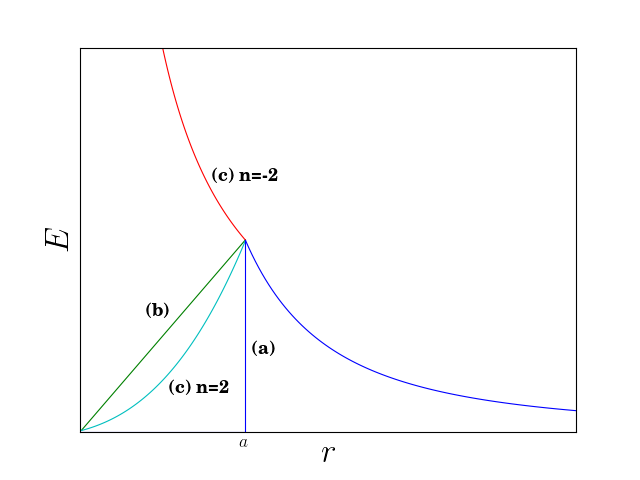
\includegraphics[scale=0.44]{problema3fig1}
 \caption{Comportamiento de los campos eléctrico obtenidos como 
una función del radio para las primeras dos esfera, y para la tercera 
con $n= -2,+2$. Recordamos que en todos los casos para $r>a$ el comportamiento 
es el mismo.}
 \label{fig:problema3fig1}
\end{figure}

\newpage

\section{Problema 4. Problema 1.5 de Classical Electrodynamics (3ra ed) de 
Jackson \cite{jackson}.}

El potencial promedio en el tiempo de un átomo de hidrógeno neutro está dado por 

$$
\Phi = \frac{q}{4\pi\epsilon_0}\frac{\euler^{-\alpha r}}{r}\left(1 + 
\frac{\alpha r}{2}\right),
$$

donde $q$ es la magnitud de la carga electrónica, y $\alpha^{-1} = a_0/2$, siendo 
$a_0$ el radio de Bohr. Encuentre la distribución de carga (tanto continua como 
discreta) que dará este potencial e interpreta tu resultado físicamente.

\vspace{.3cm}

\underline{Solución:} \vspace{.3cm}

El potencial con el que debemos trabajar es, 

\begin{equation}
 \Phi = \frac{q}{4\pi\epsilon_0}\frac{\euler^{-\alpha r}}{r}\left(1 + 
\frac{\alpha r}{2}\right).
\label{eq:potencialhidrogeno}
\end{equation}

Claramente para resolver este problema debemos utilizar la ecuación de Poisson, ya 
que ésta relaciona la densidad de carga con el potencial escalar eléctrico que 
crea. En este caso la utilizaremos para encontrar la densidad de carga. Debemos entonces 
utilizar la ecuación, 

\begin{equation}
 \nabla^2 \Phi = - \frac{\rho}{\epsilon_0},
\end{equation}

hacer la diferenciación (en coordenadas esféricas) y resolver para $\rho$. En coordenadas 
esféricas, escribimos esta ecuación como 

\begin{equation}
 \frac{1}{r^2}\frac{\partial}{\partial r}\left(r^2\frac{\partial \Phi}{\partial r}\right) +
 \frac{1}{r^2\sen{\theta}}\frac{\partial}{\partial \theta}
 \left(\sen{\theta}\frac{\partial \Phi}{\partial \theta} \right) + 
 \frac{1}{r^2\sen^2{\theta}}\frac{\partial \Phi}{\partial \phi} = 
 - \frac{\rho}{\epsilon_0}.
 \label{eq:nablaesferica}
\end{equation}

Debido a que $\Phi$ solo depende de $r$, vemos que el potencial tiene una simetría 
esférica, y por lo tanto se harán cero todas las parciales de \eqref{eq:nablaesferica} 
menos la componente radial. Es decir, 

\begin{equation}
 \frac{1}{r^2}\frac{\partial}{\partial r}\left(r^2\frac{\partial \Phi}{\partial r}\right) = 
 - \frac{\rho}{\epsilon_0}.
\end{equation}

Evaluando esta ecuación sustituyendo \eqref{eq:potencialhidrogeno}, resulta en 

\begin{align*}
  \frac{1}{r^2}\frac{\partial}{\partial r}
 \left\{r^2\frac{\partial}{\partial r}\left[\frac{q}{4\pi\epsilon_0}
 \frac{\euler^{-\alpha r}}{r}\left(1 + \frac{1}{2}\alpha r\right)\right] \right\} &= 
 - \frac{\rho}{\epsilon_0} \\
 %
 \frac{q}{4\pi\epsilon_0}\frac{1}{r^2}\frac{\partial}{\partial r}
 \left[r^2\frac{\partial}{\partial r}\left(\frac{\euler^{-\alpha r}}{r}\right) 
 + r^2\frac{\partial}{\partial r}\left(\frac{\alpha}{2}\euler^{-\alpha r}\right)
 \right] &= - \frac{\rho}{\epsilon_0} \\
 %
  \frac{q}{4\pi\epsilon_0}\frac{1}{r^2}\frac{\partial}{\partial r}
  \left[r^2\left(\frac{1}{r}\frac{\partial}{\partial r}\euler^{-\alpha r}
  + \euler^{-\alpha r}\frac{\partial}{\partial r}\frac{1}{r}\right)
  - \frac{\alpha^2}{2}r^2\euler^{-\alpha r}\right] &= - \frac{\rho}{\epsilon_0} \\
 %
  \frac{q}{4\pi\epsilon_0}\frac{1}{r^2}\frac{\partial}{\partial r}
  \left(-\alpha r \euler^{-\alpha r} + r^2\euler^{-\alpha r} 
  \frac{\partial}{\partial r}\frac{1}{r} - \frac{\alpha^2}{2}r^2\euler^{-\alpha r}
  \right) &= - \frac{\rho}{\epsilon_0} \\
 %
  \frac{q}{4\pi\epsilon_0}\left(-\frac{\alpha}{r^2}\euler^{-\alpha r} 
  \frac{\alpha^3}{2}\euler^{-\alpha r}\right) + \frac{q}{4\pi\epsilon_0}
  \frac{1}{r^2}\frac{\partial}{\partial r}\left(r^2\euler^{-\alpha r} 
  \frac{\partial}{\partial r}\frac{1}{r}\right) &= - \frac{\rho}{\epsilon_0}, 
\end{align*}

y resolviendo para $\rho$ tenemos que 

\begin{equation}
 \rho = - \frac{q\alpha^3}{8\pi}\euler^{-\alpha r} - 
 \euler^{-\alpha r}\frac{q}{4\pi}\frac{1}{r^2}\frac{\partial}{\partial r}
 \left(r^2\frac{\partial}{\partial r}\frac{1}{r} \right).
 \label{eq:rhohidrogeno1}
\end{equation}

Ahora debemos tomar en consideración algo que afecta tanto como al potencial dado,
como a la expresión que obtuvimos para $\rho$, y es que $1/r$ se hace infinito en 
el origen. Entonces debemos estudiar el comportamiento de $\rho$ pata $r \approx 
0$ y para $r > 0$. 

\vspace{.3cm}

Comencemos por el comportamiento para $r > 0$. Para $r > 0$, al evaluar las derivadas 
en el lado derecho de \eqref{eq:rhohidrogeno1} el término de la derecha se hace 
cero y nos queda 

\begin{equation}
 \rho = - \frac{q\alpha^3}{8\pi}\euler^{-\alpha r}. 
 \label{eq:rhohidrogeno2}
\end{equation}

Ahora si $r \approx 0$ tenemos que $\euler^{-\alpha r} \approx 1$ y entonces 
nos queda 

\begin{equation}
\rho = - \frac{q\alpha^3}{8\pi}- 
 \frac{q}{4\pi}\frac{1}{r^2}\frac{\partial}{\partial r}
 \left(r^2\frac{\partial}{\partial r}\frac{1}{r} \right),
\end{equation}

y usando la relación 

\begin{equation}
 \nabla^2\left(\frac{1}{r} \right) = - 4\pi \delta(r),
\end{equation}

que en este caso se lee como 

\begin{equation}
 \frac{1}{r^2}\frac{\partial}{\partial r}\left[r^2\frac{\partial}{\partial r}
 \left(\frac{1}{r} \right)\right] = - 4\pi \delta(r),
\end{equation}

y por lo tanto para $r \approx 0$, 

\begin{equation}
 \rho = - \frac{q\alpha^3}{8\pi} + q\delta(r).
 \label{eq:rhohidrogeno3}
\end{equation}

Ahora debido a que la delta es cero en todas partes menos en el origen, y debido 
a que el primer término de ecuación \eqref{eq:rhohidrogeno3} es igual al término 
de \eqref{eq:rhohidrogeno2} cuando $r=0$, podemos combinar ambos casos en 

\begin{equation}
 \boxed{\rho = - \frac{q\alpha^3}{8\pi}\euler^{-\alpha r} + q\delta(r)}.
\end{equation}

Y esta ecuación es válida para toda $r$. La parte discreta de esta ecuación
representa físicamente a un  protón estacionario con carga $q$, y al rededor de 
este protón orbita un electrón  de carga $-q$. La parte continua de la densidad 
de carga se puede interpretar como una distribución estadística de la
localización del electrón.

\newpage

\section{Problema 5. Problema 1.6 de Classical Electrodynamics (3ra ed) de 
Jackson \cite{jackson}.}

Un capacitor simple es un dispositivo formado por dos conductores aislados 
adyacentes el uno del otro. Si cargas iguales y opuestas se colocan en los 
conductores, habrá una cierta diferencia de potencial entre ellos. La razón de 
la magnitud de la carga en un conductor a la magnitud de la diferencia de 
potencial es llamada capacitancia (en unidades SI se mide en faradios). Usando la 
ley de Gauss, calcule la capacitancia de 

\begin{enumerate}[label=\textbf{(\alph*)}]
 \item dos láminas grandes, planas, de área $A$, separadas por una pequeña 
 distancia $d$;
 \item dos esferas concéntricas conductoras con radios $a,b$ $(b > a)$;
 \item dos cilindros concéntricos conductores de longitud $L$, grande comparada 
 a sus radios $a,b$ $(b > a)$.
 \item ¿Cuál es el diámetro interno del conductor externo en un cable coaxial 
 lleno de aire, cuyo conductor central es un alambre cilíndrico de diámetro 
 1 mm y cuya capacitancia es $3\times 10^{-11}$ F/m? ¿$3\times 10^{-12}$ F/m?
\end{enumerate}

\vspace{.3cm}

\underline{Solución:} \vspace{.3cm}

La técnica que utilizaremos para calcular la capacitancia en todos los casos será, 
asumir cargas $\pm Q$ en los conductores, luego utilizando la ley de Gauss encontratemos 
$E$ en función de $Q$, 

\begin{equation}
 \oint \mathbf{E} \cdot d\mathbf{a} = \frac{1}{\epsilon_0}\int_V \rho(x)d^3x = 
 \frac{Q}{\epsilon_0},
\end{equation}

luego, se calcula la diferencia de potenciales $V$ entre los dos conductores con 

\begin{equation}
 \int_A^B \mathbf{E} \cdot d\mathbf{l} = - (\Phi_B - \Phi_A),
\end{equation}

y por último se calcula la capacitancia con 

\begin{equation}
 C = \left|\frac{Q}{V}\right|.
\end{equation}

\textbf{(a)} Para resolver el primer inciso, colocamos una carga $-Q$ en una lámina 
en $z=0$ y una carga $+Q$ en la otra lámina en $z=d$, entonces una diferencia de 
voltaje constante se establece entre las mismas. Recordando que utilizando el método 
de Gauss obtenemos que para las láminas (como son muy grandes, y separadas por una 
distancia pequeña podemos aproximarlas como infinitas), ya sumada la contribución de 
cada una será 

\begin{equation}
 E = \frac{\sigma}{\epsilon_0} = \frac{Q}{A\epsilon_0},
\end{equation}

y por otra parte, la diferencia de potencial entre las láminas (por construcción) 
será simplemente $V = Ed$, es decir que 

\begin{equation}
 V = \frac{Qd}{A\epsilon_0},
\end{equation}

por lo tanto la capacitancia será 

\begin{equation}
 \boxed{C = \frac{Q}{V} = \frac{\epsilon_0 A}{d}}.
\end{equation}

\textbf{(b)} En el segundo inciso colocamos una carga $+Q$ en la esfera de 
radio $a$ y otra de $-Q$ en la esfera de radio $b$. Si recordamos, usando el método 
de Gauss y dibujando una esfera de integración de radio $r$ tal que $a < r < b$, 
por simetría obtenemos que el campo eléctrico sólo no es cero entre las dos 
esferas, y tiene una magnitud de 

\begin{equation}
 E = \frac{Q}{4\pi\epsilon_0}\frac{1}{r^2},
\end{equation}

luego tenemos que 

\begin{equation}
 V = - \int_a^b E dr = \frac{Q}{4\pi\epsilon_0}\left(\frac{1}{a} - \frac{1}{b}\right),
\end{equation}

y por lo tanto 

\begin{equation}
 \boxed{C = \frac{Q}{V} = 4\pi\epsilon_0\left(\frac{1}{a} - \frac{1}{b}\right)}.
\end{equation}

\textbf{(c)} En el tercer inciso colocamos una carga $+Q$ en el cilindro de radio 
$a$ y una carga $-Q$ en el cilindro de radio $b$. De nuevo, utilizando el método 
gaussiano, dibujamos una superficie de integración cilíndrica de radio $r$ tal que 
$a < r < b$, usamos la simetría, y obtenemos que 

\begin{equation}
 E = \frac{Q}{2\pi\epsilon_0 L}\frac{1}{r},
\end{equation}

donde $L$ es la longitud del cilindro de radio $r$. Luego tenemos que 

\begin{equation}
 V = - \int_a^b E dr = \frac{Q}{2\pi\epsilon_0 L}\ln{\frac{a}{b}},
\end{equation}

y por lo tanto 

\begin{equation}
 \boxed{C = \frac{Q}{V} = 2\pi\epsilon_0 L \left(\ln{\frac{a}{b}} \right)^{-1}}.
\end{equation}

\textbf{(d)} En este inciso, debemos resolver para $2b$ la ecuación para la capacitancia 
del inciso anterior y luego sustituir los valores dados. Con el valor que 
nos dan que $2a = 1$ mm, y valores especificados para la capacitancia por unidad 
de distancia $(C/L)$, resolviendo para $2b$ tenemos 

\begin{equation}
 2b = 2a\exp\left(\frac{2\pi\epsilon_0}{C/L}\right),
\end{equation}

para $C/L = 3 \times 10^{-11}$ F/m tenemos que el diámetro interno, $(2b)$, del 
cable debe ser de $\boxed{6.4 \text{ mm}}$, mientras que para $C/L = 3 \times 10^{-12}$ F/m tenemos 
que el diámetro interno, $(2b)$, del cable debe ser tan grande como 
de $\boxed{113 \text{ km}}$. Con lo que vemos que para propósitos prácticos, la capacitancia 
por unidad de longitud de un cable coaxial no puede ser mucho más pequeña que 
unos pocos $10^{-11}$ F/m.

\newpage

\begin{thebibliography}{10}
\bibitem{jackson}
J. Jackson, \emph{Classical Electrodynamics}, 3ra edición. John Wiley and Sons, Inc. 
1999.
\end{thebibliography}

\end{document}